\documentclass[10pt]{article}\usepackage[margin=.65in]{geometry}\usepackage[T1]{fontenc}\usepackage{graphicx}\setlength{\parindent}{0pt}\setlength{\parskip}{7pt}\sloppy\begin{document}{\large Constructed quintic fallback reduction trace}\par Producer proof packet, 2026-11-01. Independent review of this new component is pending.\par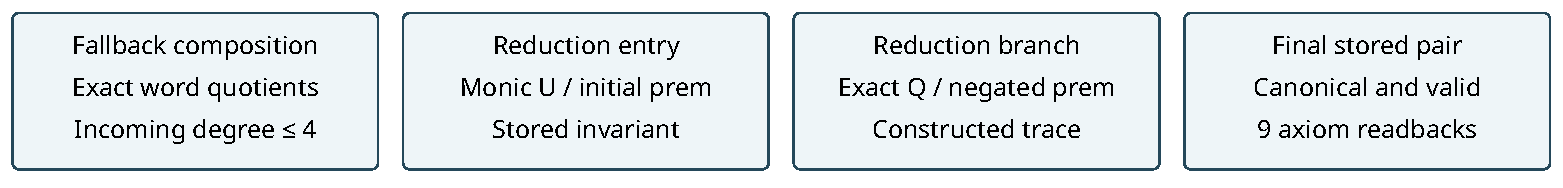
\includegraphics[width=\linewidth]{diagram.pdf}\par Result. The modeled reduction now constructs its exact quotient and remainder rather than assuming their properties. From canonical normalized nonzero U, canonical V, a degree-five curve polynomial, degree(U) at most four, and U dividing f-V squared, the entry theorem normalizes U, computes the initial remainder, and constructs a Run ending in a canonical valid pair that fits the final arrays. The proof constructs either a stop branch or one quotient/remainder step followed by a stop branch.

Step. The residual is computed by the modeled psub and polynomial multiplication. Exact division constructs Q and proves its decoded quotient identity and canonical normalized storage. The quintic bound makes Q nonzero of degree at most two. Monic normalization produces the new U. The modeled remainder of pneg(V) by new U is canonical and normalized, strictly shorter than new U, and preserves the residual divisibility. The final pair satisfies the formal Mumford-validity predicate and fixed-storage bounds.

Fallback endpoint. The previously constructed two EEA runs and exact fallback divisions produce U, W and the first remainder R. The exact identity Ua*Ub=U*D squared, with nonzero input polynomials of degree at most two, implies nonzero U and degree(U) at most four. Composing this with reduction constructs the initial normalized remainder and final Run, canonical output coefficient lists, nonempty U, at most three U coefficients and at most two V coefficients. No resultant or smoothness heuristic is used for these algebraic/storage claims.

Checks. Six fresh modules, five main declarations, four fixed controls and nine exact named axiom readbacks passed. The false theorem exits one; the native checker rejects forbidden axioms, empty readback and a wrong name. All successful fresh checks preserve their bound inputs. Fixed controls exercise constant and quadratic stop branches, the cubic length guard and zero negation. An initial loop proof attempt needed the empty polynomial degree rewritten explicitly; that failed receipt is retained. Dependency caches are reused, and no independent fresh kernel replay is claimed.

Assumptions and native scope. Prime p with 1 $<$ p $<$ 2\textasciicircum{}31; canonical input coefficients; normalized nonzero input U polynomials; both input residual divisibilities; degree at most two for each input U and degree five for f. The native correspondence concerns Field.n == 1 with diagnostic tables absent, as in the relevant constructor Field::new(p,1,0). General extension-field dispatch, table-backed dispatch, physical allocation, counter events, array-copy semantics and compiled Rust equivalence are not proved by this word-list model. Divisor-class interpretation remains a separate obligation.

Independent predecessor review. A separate reviewer found the ten declarations of quintic-reduction-storage faithful at their stated conditional scope. The reviewer inspected fourteen named readbacks but did not perform fresh kernel replay and inherited producer context; this was not a mutually blind re-derivation. The complete note is archived here. Two requested clarifications are explicit above: native field dispatch, and the distinction between decoded validity for an arbitrary supplied remainder and canonical storage. The new construction proves canonicality of the remainder it actually computes. The predecessor review does not review these new theorems.

Source and prior work. Native src/cryptanalysis/three\_leads.rs at 2bf73d8b6b78918aa31c5ec1abfd16d221449f20, fallback branch and reduce control flow; native source unchanged from fe44742979. Prior quintic-reduction-storage, fallback-geometric-invariant, fallback-word-divisions and pegcd-six-word-endpoint packets supply the component lemmas. Standard pinned Mathlib product-degree identities supply the composition degree bound. No novelty or performance claim is made.

Next joint. Independently review the constructed call wiring and Run relation, bind the prime-field runtime dispatch explicitly, and establish the divisor-class meaning of the returned pair. This packet covers the generic fallback route, not the optimized addition branches. The frozen 1,260-target scope and expired campaign deadline are preserved. No scientific run or fresh cost ratio is reported.
\end{document}